%%%%%%%%%%%%%%%%%%%%% {{{
%%Options for presentations (in-class) and handouts (e.g. print).
\documentclass[pdf,9pt]{beamer}
% \documentclass[pdf,9pt]{beamer}


%%%%%%%%%%%%%%%%%%%%%%
%Change this for different slides so it appears in bar
\usepackage{authoraftertitle}
\date{Chapter 4. Vector Geometry\\ \S 4-2. Projections and Planes}

%%%%%%%%%%%%%%%%%%%%%%
%% Upload common style file
\usepackage{LyryxLAWASlidesStyle}

\begin{document}

%%%%%%%%%%%%%%%%%%%%%%%
%% Title Page and Copyright Common to All Slides

%Title Page
\input frontmatter/titlepage.tex

%LOTS Page
\input frontmatter/lyryxopentexts.tex

%Copyright Page
\input frontmatter/copyright.tex

%%%%%%%%%%%%%%%%%%%%%%%%% }}}
%-------------- start slide -------------------------------%{{{ 2
\begin{frame}[fragile]
   \tableofcontents
\end{frame}
%-------------- end slide -------------------------------%}}}
\Chapter4Note
\section[\textcolor{yellow}{}]{\textcolor{yellow}{The Dot Product and Angles}}
%-------------- start slide -------------------------------%{{{ 4
\frame{
\frametitle{The Dot Product and Angles}
\pause
\begin{definition}
    Let $\vec{u}=
    \left[\begin{array}{c}
    x_1 \\ y_1 \\ z_1
    \end{array}\right]$ and
    $\vec{v}=
    \left[\begin{array}{c}
    x_2 \\ y_2 \\ z_2
    \end{array}\right]$ be vectors in $\RR^3$.
    The \alert{dot product} of $\vec{u}$ and $\vec{v}$ is
    \[ \vec{u}\dotprod\vec{v}=x_1x_2 + y_1y_2 + z_1z_2,\]
    i.e., $\vec{u}\dotprod\vec{v}$ is a \alert{scalar}.
\end{definition}
\vfill
\pause

\begin{remark}
  Another way to think about the dot product is as the
  $1\times 1$ matrix
  \[ \vec{u}^T\vec{v}
  =
  \left[\begin{array}{ccc}
  x_1 & y_1 & z_1
  \end{array}\right]
  \left[\begin{array}{c}
  x_2 \\ y_2 \\ z_2
  \end{array}\right]
  =
  \left[\begin{array}{c}
  x_1x_2 + y_1y_2 + z_1z_2
  \end{array}\right] .\]
\end{remark}
}
%-------------- end slide -------------------------------%}}}
%-------------- start slide -------------------------------%{{{ 5
\frame{
\begin{theorem}[ Properties of the Dot Product ]
    Let $\vec{u}, \vec{v}, \vec{w}$ be vectors in $\RR^3$
    (or $\RR^2$) and let $k\in\RR$.
    \begin{enumerate}
	\item<2-> $\vec{u}\dotprod\vec{v}$ is a real number.
	\item<3-> $\vec{u}\dotprod\vec{v}=\vec{v}\dotprod\vec{u}$.  \hfill (commutative property)
	\item<4-> $\vec{u}\dotprod\vec{0}=0$.
	\item<5-> $\vec{u}\dotprod\vec{u}=||\vec{u}||^2$.
	\item<6-> $(k\vec{u})\dotprod\vec{v}= k(\vec{u}\dotprod\vec{v})= \vec{u}\dotprod(k\vec{v})$.  \hfill (associative property)
	\item<7-> $\vec{u}\dotprod(\vec{v} + \vec{w}) = \vec{u}\dotprod\vec{v} + \vec{u}\dotprod\vec{w}$.  \hfill (distributive properties)

	$\vec{u}\dotprod(\vec{v} - \vec{w}) =
	\vec{u}\dotprod\vec{v} - \vec{u}\dotprod\vec{w}$.
    \end{enumerate}
\end{theorem}
}
%-------------- end slide -------------------------------%}}}
%-------------- start slide -------------------------------%{{{ 6
{
\frame{

\begin{emptytitle}
    Let $\vec{u}$ and $\vec{v}$ be two vectors in $\RR^3$ (or $\RR^2$).
    There is a unique angle $\theta$ between $\vec{u}$ and $\vec{v}$
    with $0\leq\theta\leq\pi$.
\end{emptytitle}

\begin{picture}(4,.9)
% \put(0.8,0.1){
\includegraphics[scale=.8]{figures/vectors-14_copy.pdf}}
% \put(0.8,0.2){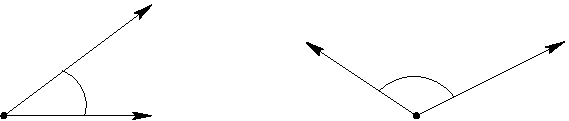
\includegraphics[scale=.8]{figures/vectors-14.pdf}}
\put(0.8,0.0){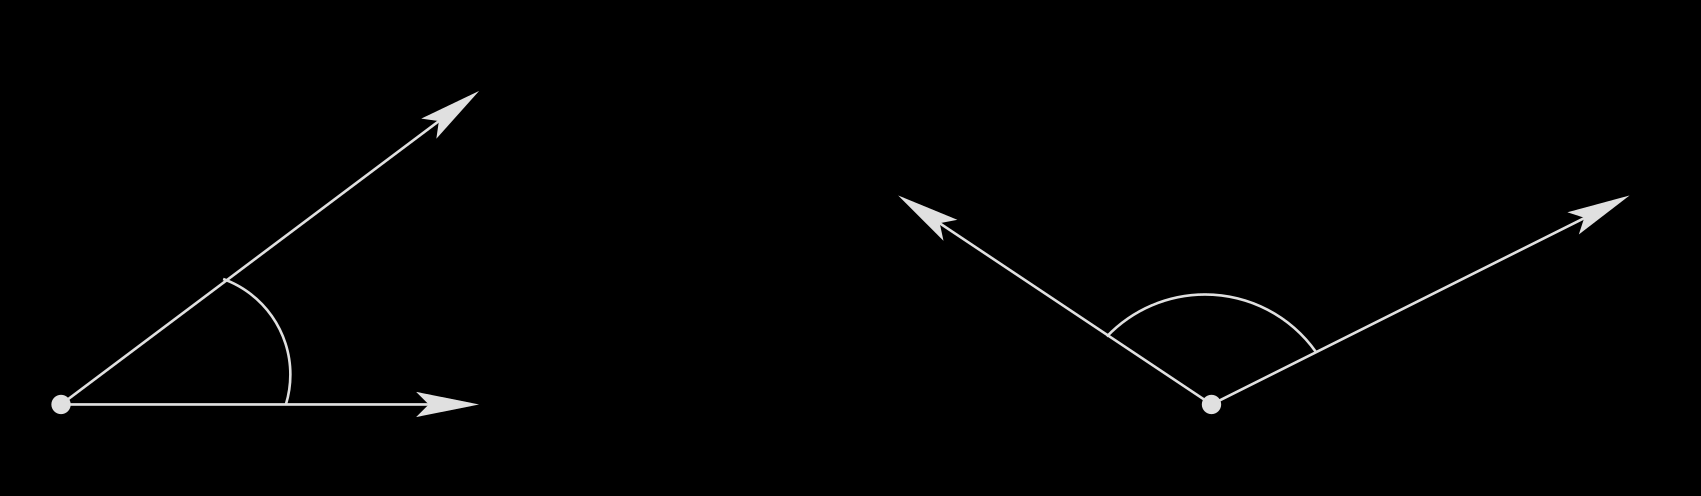
\includegraphics[scale=.13]{figures/vectors-14.png}}
\put(1.1,0.45){\small $\vec{u}$}
\put(1.1,0.0){\small $\vec{v}$}
\put(1.4,0.3){\small $\theta$}
\put(2.6,0.2){\small $\vec{u}$}
\put(3.4,0.2){\small $\vec{v}$}
\put(3.0,0.4){\small $\theta$}
\end{picture}
\vfill
\pause
\begin{theorem}
    Let $\vec{u}$ and $\vec{v}$ be nonzero vectors, and let
    $\theta$ denote the angle between $\vec{u}$ and $\vec{v}$.
    Then
    \[ \vec{u}\dotprod\vec{v} = ||\vec{u}||~||\vec{v}||\cos\theta.\]
\end{theorem}
\vfill \pause
}
%-------------- end slide -------------------------------%}}}
%-------------- start slide -------------------------------%{{{ 7
\begin{frame}[fragile]
 \begin{proofnoend}
   We first prove the \alert{Law of Cosines} -- a generalization of the {\it Pythagorean theorem}:
   \begin{center}
     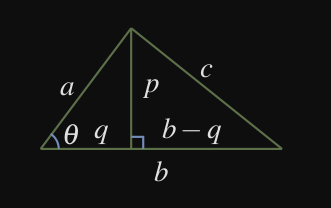
\includegraphics[scale=0.25]{./figures/Low-Cosine.png}
   \end{center}
   \begin{align*}
     c^2 = p^2 +\left(b-q\right)^2 &= a^2 \sin^2\theta + \left(b-a\cos\theta\right)^2\\
                                   &= a^2 \left(\sin^2\theta+ \cos^2\theta\right) + b^2 -2ab\cos\theta\\
                                   &= a^2 +b^2 -2ab\cos\theta.
   \end{align*}
 \end{proofnoend}
\end{frame}
%-------------- end slide -------------------------------%}}}
%-------------- start slide -------------------------------%{{{ 8
\begin{frame}[fragile]
    \begin{proofnoend}[continued]
   In terms of vectors, we see that
   \begin{center}
     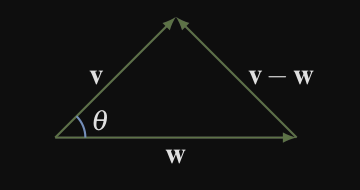
\includegraphics[scale=0.25]{./figures/InnerProduct.png}
   \end{center}
   \begin{align*}
     ||\vec{v} -\vec{w}||^2 = ||\vec{v}||^2 + ||\vec{w}||^2 - 2 ||\vec{v}||\: ||\vec{w}|| \cos \theta
   \end{align*}
   \vspace{-3em}
   \pause
   \begin{align*}
       || & \\
	  &\hspace{-2em}\left(\vec{v}-\vec{w}\right) \cdot \left(\vec{v}-\vec{w}\right) = ||\vec{v}||^2 - 2 \vec{v}\cdot \vec{w} + ||\vec{w}||^2
   \end{align*}
   \vspace{-2em}
   \pause
   \[\Downarrow\]
   \vspace{-2em}
    \begin{align*}
	||\vec{v}||^2 + ||\vec{w}||^2 - 2 ||\vec{v}||\: ||\vec{w}|| \cos \theta  = ||\vec{v}||^2 - 2 \vec{v}\cdot \vec{w} + ||\vec{w}||^2
    \end{align*}
   \vspace{-2em}
   \[\Downarrow\]
   \vspace{-1.5em}
    \pause
    \[ \vec{u}\dotprod\vec{v} = ||\vec{u}||~||\vec{v}||\cos\theta.\]
    \myQED
 \end{proofnoend}
\end{frame}
%-------------- end slide -------------------------------%}}}
%-------------- start slide -------------------------------%{{{ 9
\frame{
\[ \vec{u}\dotprod\vec{v} = ||\vec{u}||~||\vec{v}||\cos\theta.\]
\smallskip

\begin{itemize}
    \item<2-> If $0\leq\theta <\frac{\pi}{2}$, then $\cos\theta >0$.
    \item<3-> If $\theta=\frac{\pi}{2}$, then $\cos\theta =0$.
    \item<4-> If $\frac{\pi}{2}<\theta\leq\pi$, then $\cos\theta <0$.
\end{itemize}
\bigskip

\uncover<5->{Therefore, for nonzero vectors
$\vec{u}$ and $\vec{v}$,
\begin{itemize}
    \item<5-> $\vec{u}\dotprod\vec{v}>0$ if and only if $0\leq\theta\ < \frac{\pi}{2}$.
    \item<6-> $\vec{u}\dotprod\vec{v}=0$ if and only if $\theta=\frac{\pi}{2}$.
    \item<7-> $\vec{u}\dotprod\vec{v}<0$ if and only if $\frac{\pi}{2}<\theta\leq\pi$.
\end{itemize}}
}
%-------------- end slide -------------------------------%}}}
%-------------- start slide -------------------------------%{{{ 10
\frame{
\begin{definition}
    Vectors $\vec{u}$ and $\vec{v}$ are \alert{orthogonal}
    if and only if $\vec{u}=\vec{0}$ or $\vec{v}=\vec{0}$
    or $\theta=\frac{\pi}{2}$.
\end{definition}
\bigskip

\uncover<2->{
\begin{theorem}
    Vectors $\vec{u}$ and $\vec{v}$ are orthogonal if
    and only if $\vec{u}\dotprod\vec{v}=0$.
\end{theorem}}
}
%-------------- end slide -------------------------------%}}}
%-------------- start slide -------------------------------%{{{ 11
\frame{
\begin{problem}
    Find the angle between
    $\vec{u}=
    \left[\begin{array}{r}
    1 \\ 0 \\ -1
    \end{array}\right]$
    and
    $\vec{v}=
    \left[\begin{array}{r}
    0 \\ 1 \\ -1
    \end{array}\right]$.
\end{problem}
\vfill
\pause
\begin{solution}
    $\vec{u}\dotprod\vec{v}=1$,
    $||\vec{u}||=\sqrt{2}$ and $||\vec{v}||=\sqrt{2}$.

    Therefore,
    \[ \cos\theta = \frac{\vec{u}\dotprod\vec{v}}
	{||\vec{u}||~||\vec{v}||}
    = \frac{1}{\sqrt{2}\sqrt{2}}=\frac{1}{2}.  \]

    Since $0\leq\theta\leq\pi$,
    $\theta = \frac{\pi}{3}$.
    \bigskip

    Therefore, the angle between $\vec{u}$ and $\vec{v}$ is
    $\frac{\pi}{3}$.
\end{solution}
}
%-------------- end slide -------------------------------%}}}
%-------------- start slide -------------------------------%{{{ 12
\frame{
\begin{problem}
    Find the angle between
    $\vec{u}=
    \left[\begin{array}{r}
    7 \\ -1 \\ 3
    \end{array}\right]$
    and
    $\vec{v}=
    \left[\begin{array}{r}
    1 \\ 4 \\ -1
    \end{array}\right]$.
\end{problem}
\medskip
\vfill
\begin{solution}
    $\vec{u}\dotprod\vec{v}=0$,
    and therefore the angle between the vectors is $\frac{\pi}{2}$.
\end{solution}
}
%-------------- end slide -------------------------------%}}}
%-------------- start slide -------------------------------%{{{ 13
\frame{
\begin{problem}
    \hspace{-1em}
    Find all vectors $\vec{v}=
    \left[\begin{array}{r}
    x \\ y \\ z
    \end{array}\right]$
    orthogonal to both
    $\vec{u}=
    \left[\begin{array}{r}
    -1 \\ -3 \\ 2
    \end{array}\right]$ and $\vec{w}=
    \left[\begin{array}{r}
    0 \\ 1 \\ 1
    \end{array}\right]$.
\end{problem}
\pause
\vfill
\begin{solution}
    There are infinitely many such vectors.
    \pause
    Since $\vec{v}$ is orthogonal to both $\vec{u}$ and $\vec{w}$,
    \[ \begin{array}{rcl}
	\vec{v}\dotprod\vec{u} & = & -x-3y+2z=0 \\
	\vec{v}\dotprod\vec{w} & = & y+z=0
    \end{array}\]
\end{solution}
}
%-------------- end slide -------------------------------%}}}
%-------------- start slide -------------------------------%{{{ 14
\begin{frame}[fragile]
    \begin{solution}[continued]
	This is a homogeneous system of two linear equation in three
	variables.
	\[
	    \left[\begin{array}{rrr|r}
		    -1 & -3 & 2 & 0 \\
		    0 & 1 & 1 & 0
	    \end{array}\right]
	    \rightarrow \cdots \rightarrow
	    \left[\begin{array}{rrr|r}
		    1 & 0 & -5 & 0 \\
		    0 & 1 & 1 & 0
	    \end{array}\right]
	\]
	\\
	Therefore,
	$\vec{v}=t\left[\begin{array}{r}
	5 \\ -1 \\ 1
	\end{array}\right]$ for all $t\in\RR$.
   \end{solution}
\end{frame}
%-------------- end slide -------------------------------%}}}
%-------------- start slide -------------------------------%{{{ 15
\frame{
\begin{problem}
    Are $A(4,-7,9)$, $B(6,4,4)$ and $C(7,10,-6)$ the vertices of
    a right angle triangle?
\end{problem}
\vfill
\pause
\begin{solution}
    \[
    \overrightarrow{AB} =
    \left[\begin{array}{r}
    2 \\ 11 \\ -5
    \end{array}\right],\quad
    \overrightarrow{AC} =
    \left[\begin{array}{r}
    3 \\ 17 \\ -15
    \end{array}\right],\quad
    \overrightarrow{BC} =
    \left[\begin{array}{r}
    1 \\ 6 \\ -10
    \end{array}\right] \]
    \pause

    \begin{itemize}
    \item $\overrightarrow{AB}\dotprod \overrightarrow{AC} = 6 + 187 + 75 \neq 0$.\\[0.5em] \pause
    \item $\overrightarrow{BA}\dotprod \overrightarrow{BC} = (-\overrightarrow{AB})\dotprod \overrightarrow{BC} = -2 -66-50 \neq 0$.\\[0.5em] \pause
    \item $\overrightarrow{CA}\dotprod \overrightarrow{CB} = (-\overrightarrow{AC})\dotprod (-\overrightarrow{BC}) = \overrightarrow{AC}\dotprod \overrightarrow{BC} =3+102+150\neq 0$.
    \end{itemize}
    \pause
    Because none of the angles is $\frac{\pi}{2}$, the triangle is not a right angle triangle.
 \end{solution}
}
%-------------- end slide -------------------------------%}}}
%-------------- start slide -------------------------------%{{{ 16
\frame{
\begin{problem}
    A rhombus is a parallelogram with sides of equal length.
    Prove that the diagonals of a rhombus are perpendicular.
\end{problem}
\vfill
\pause
\begin{solution}
    \begin{picture}(4,.9)
	\put(0.4,0.1){
\includegraphics[scale=.8]{figures/vectors-15_copy.pdf}}
	\put(0.5,0.5){\small $\vec{u}$}
	\put(0.8,0.0){\small $\vec{v}$}
	\put(1.7,0.8){\small Define the parallelogram (rhombus) by }
	\put(1.7,0.6){\small vectors $\vec{u}$ and $\vec{v}$.}
	\put(1.7,0.3){\small Then the diagonals are $\vec{u}+\vec{v}$
	and $\vec{u}-\vec{v}$.}
	\put(1.7,0.0){\small Show that $\vec{u}+\vec{v}$ and
	$\vec{u}-\vec{v}$ are perpendicular.}
    \end{picture}
    \pause
    \begin{eqnarray*}
    (\vec{u}+\vec{v})\dotprod(\vec{u}-\vec{v}) & = & \vec{u}\dotprod\vec{u}-\vec{u}\dotprod\vec{v} + \vec{v}\dotprod\vec{u} -\vec{v}\dotprod\vec{v} \\
                                               & = & ||\vec{u}||^2 -\vec{u}\dotprod\vec{v} + \vec{u}\dotprod\vec{v} - ||\vec{v}||^2                 \\
                                               & = & ||\vec{u}||^2 - ||\vec{v}||^2                                                                  \\
                                               & = & 0, \qquad \mbox{ since } ||\vec{u}||=||\vec{v}||.
    \end{eqnarray*}
    Therefore, the diagonals are perpendicular.
\end{solution}
}
%-------------- end slide -------------------------------%}}}
\section[\textcolor{yellow}{}]{\textcolor{yellow}{Projections}}
%-------------- start slide -------------------------------%{{{ 17
\frame{
\frametitle{Projections}
\pause
\begin{emptytitle}
    Given two nonzero vectors $\vec{u}$ and $\vec{d}$, one can always express $\vec{u}$ as a sum
    $\vec{u}=\vec{u}_1 + \vec{u}_2$, where $\vec{u}_1$ is parallel to $\vec{d}$ and
    $\vec{u}_2$ is orthogonal to $\vec{d}$.
\end{emptytitle}
\vfill
\pause
\begin{picture}(3,.9)
    \put(0.3,0.1){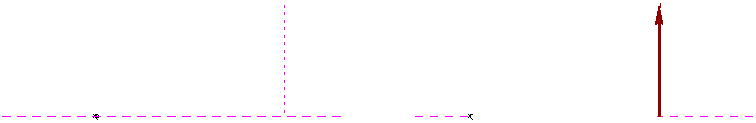
\includegraphics[scale=.8]{figures/vectors-16_copy.pdf}}
    % \put(0.3,0.2){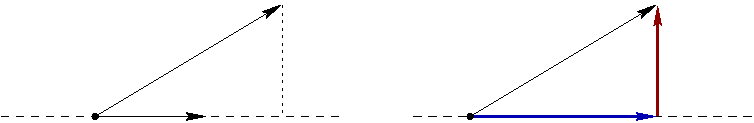
\includegraphics[scale=.8]{figures/vectors-16.pdf}}
    \put(1.05,-0.05){\small $\vec{d}$}
    \put(1.25,0.5){\small $\vec{u}$}
    \put(3.25,0.0){\small $\vec{u}_1$}
    \put(3.25,0.5){\small $\vec{u}$}
    \put(3.85,0.3){\small $\vec{u}_2$}
\end{picture}
\vfill
\pause
\begin{emptytitle}
    $\vec{u}_1$ is \alert{the projection of $\vec{u}$ onto
    $\vec{d}$}, written
    $\vec{u}_1 = \proj_{\vec{d}} \vec{u}$.
\end{emptytitle}
\vfill
\pause
\begin{emptytitle}
   \begin{center}
   How to find $\vec{u}_1 = \proj_{\vec{d}} \vec{u}$~?
   \end{center}
\end{emptytitle}
}
%-------------- end slide -------------------------------%}}}
%-------------- start slide -------------------------------%{{{ 18
\begin{frame}[fragile]
\vspace{-1em}
\begin{align}
    \vec{u}_2 \dotprod\vec{u}_1                      & = 0 \tag{$\vec{u}_1\perp \vec{u}_2$ }                                     \\
    \vec{u}_2 \dotprod(t\vec{d})                     & = 0 \tag{$\vec{u}_1=t \vec{d}$}                                           \\
    t(\vec{u}_2 \dotprod\vec{d})                     & = 0 \notag                                                                \\
    \vec{u}_2 \dotprod\vec{d}                        & = 0 \tag{$t\ne 0$ b.c. $\vec{u}\ne \vec{0}  $}                            \\
    (\vec{u}-\vec{u_1})\dotprod\vec{d}               & = 0 \tag{$\vec{u}_1+\vec{u}_2=\vec{u}$}                                   \\
    \vec{u}\dotprod\vec{d}-\vec{u_1}\dotprod\vec{d}  & = 0 \notag                                                                \\
    \vec{u}\dotprod\vec{d}-(t\vec{d})\dotprod\vec{d} & = 0 \tag{$\vec{u}_1=t \vec{d}$}                                           \\
    \vec{u}\dotprod\vec{d}-t(\vec{d}\dotprod\vec{d}) & = 0 \notag                                                                \\
    \vec{u}\dotprod\vec{d}-t||\vec{d}||^2            & = 0 \notag                                                                \\
    \vec{u}\dotprod\vec{d}                           & = t||\vec{d}||^2\notag                                                    \\
    t                                                & = \frac{\vec{u}\dotprod\vec{d}}{||\vec{d}||^2} \tag{$\vec{d}\ne \vec{0}$} \\
    \vec{u}_1                                        & = \frac{\vec{u}\dotprod\vec{d}}{||\vec{d}||^2}\vec{d} \tag{$\vec{u}_1=t \vec{d}$}
\end{align}
\end{frame}
%-------------- end slide -------------------------------%}}}
%-------------- start slide -------------------------------%{{{ 19
\frame{
\begin{picture}(3,.9)
    \put(0.3,0.1){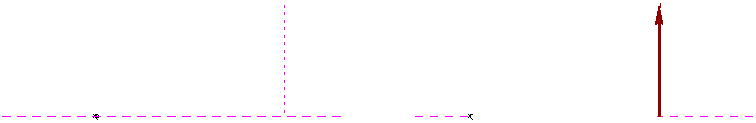
\includegraphics[scale=.8]{figures/vectors-16_copy.pdf}}
    % \put(0.3,0.2){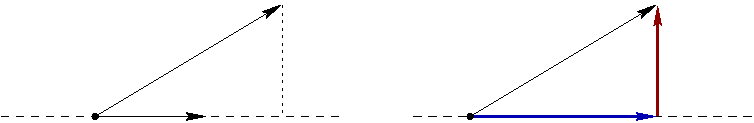
\includegraphics[scale=.8]{figures/vectors-16.pdf}}
    \put(1.05,-0.05){\small $\vec{d}$}
    \put(1.25,0.5){\small $\vec{u}$}
    \put(3.25,0.0){\small $\vec{u}_1$}
    \put(3.25,0.5){\small $\vec{u}$}
    \put(3.85,0.3){\small $\vec{u}_2$}
\end{picture}
\vfill
\pause
\begin{theorem}
    Let $\vec{u}$ and $\vec{d}$ be vectors with $\vec{d}\neq\vec{0}$.
    \begin{enumerate}
	\item<2-> The projection of $\vec{u}$ onto $\vec{d}$ is
	    \[ \vec{u}_1 = \proj_{\vec{d}}\vec{u} = \frac{\vec{u}\dotprod\vec{d}}{||\vec{d}||^2} \vec{d}.\]
	\item<3->
	    \[ \vec{u}_2 = \vec{u}-\frac{\vec{u}\dotprod\vec{d}}{||\vec{d}||^2} \vec{d}\]
	    is orthogonal to $\vec{d}$.
    \end{enumerate}
\end{theorem}
}
%-------------- end slide -------------------------------%}}}
%-------------- start slide -------------------------------%{{{ 20
\begin{frame}[fragile]
\begin{center}
    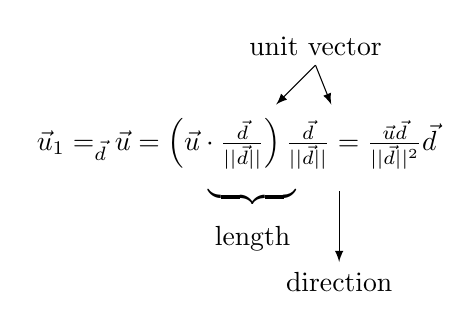
\begin{tikzpicture}[scale=1, transform shape]
	\tikzset{>=latex}
	\node at (0,0) {$\vec{u}_1 = \proj_{\vec{d}}\vec{u} = \left(\vec{u} \cdot \frac{\vec{d}}{||\vec{d}|| } \right) \frac{\vec{d}}{||\vec{d}||} = \frac{\vec{u}\dotprod\vec{d}}{||\vec{d}||^2} \vec{d}$};
	\pause
	\draw [->] (1,1) -- (0.5,0.5);
	\draw [->] (1,1) node [above] {unit vector} -- (1.2,0.5);
	\pause
	\node at (0.2,-0.6) {$\underbrace{\phantom{aaaaaa}}$};
	\node at (0.2,-1.2) {length};
	\pause
	\draw [->] (1.3,-0.6) -- (1.3,-1.5) node [below] {direction};
    \end{tikzpicture}
\end{center}
\end{frame}
%-------------- end slide -------------------------------%}}}
%-------------- start slide -------------------------------%{{{ 21
\frame{
\begin{problem}
    Let $\vec{u}=\left[\begin{array}{r}
    2 \\ -1 \\ 0 \end{array}\right]$
    and
    $\vec{v}=\left[\begin{array}{r}
    3 \\ 1 \\ -1 \end{array}\right]$.
    Find vectors $\vec{u}_1$ and $\vec{u}_2$ so that
    $\vec{u}=\vec{u}_1 + \vec{u}_2$, with
    $\vec{u}_1$ parallel to $\vec{v}$ and
    $\vec{u}_2$ orthogonal to $\vec{v}$.
\end{problem}
\vfill
\pause
\begin{solution}
    \[
    \vec{u}_1
    =\proj_{\vec{v}} \vec{u}
    = \frac{\vec{u}\dotprod\vec{v}}{||\vec{v}||^2} \vec{v}
    = \frac{5}{11} \left[\begin{array}{r} 3 \\ 1 \\ -1 \end{array}\right]
    =\left[\begin{array}{r} 15/11 \\ 5/11 \\ -5/11 \end{array}\right].
    \]
    \pause
    \[
    \vec{u}_2
    =\vec{u}-\vec{u}_1
    =\left[\begin{array}{r} 2 \\ -1 \\ 0 \end{array}\right] - \frac{5}{11} \left[\begin{array}{r} 3 \\ 1 \\ -1 \end{array}\right]
    = \frac{1}{11} \left[\begin{array}{r} 7 \\ -16 \\ 5 \end{array}\right]
    =\left[\begin{array}{r} 7/11 \\ -16/11 \\ 5/11 \end{array}\right].
    \]
\end{solution}
}
%-------------- end slide -------------------------------%}}}
%-------------- start slide -------------------------------%{{{ 22
\frame{
\begin{problem}
    % \textcolor{titletextcolour}{Example}\\[0.5em]
    Let $P(3,2,-1)$ be a point in $\RR^3$ and $L$ a line with
    equation
    \[
	\left[\begin{array}{c}
	x \\ y \\ z \end{array}\right]
	=
	\left[\begin{array}{r}
	2 \\ 1 \\ 3 \end{array}\right]
	+
	t\left[\begin{array}{r}
	3 \\ -1 \\ -2 \end{array}\right].\]
	Find the \textcolor{yellow}{shortest distance} from $P$ to $L$,
	and \textcolor{yellow}{find the point} $Q$ on $L$ that is closest to $P$.
\end{problem}
\vfill
\pause
\begin{solution}
    \begin{picture}(4,1.2)
	\put(0.2,0.2){
\includegraphics[scale=.7]{figures/vectors-17_copy.pdf}}
	\put(0.1,0.2){\small $0$}
	\put(0.2,0.7){\small $L$}
	\put(0.5,0.6){\small $P_0$}
	\put(1.65,1.05){\small $P$}
	\put(1.2,0.25){\small $Q$}
	\put(1.0,0.95){\small $\vec{u}$}
	\put(2.0,1.2){\small Let $P_0=P_0(2,1,3)$ be a point on $L$,}
	\put(2.0,1.0){\small and let
	    $\vec{d}= \left[\begin{array}{ccc}
	3 & -1 & -2 \end{array}\right]^T$.}
	\put(2.0,0.8){\small Then $\overrightarrow{P_0Q}
	    =\proj_{\vec{d}}\overrightarrow{P_0P}$,
	    $\overrightarrow{0Q}=\overrightarrow{0P_0} +
	\overrightarrow{P_0Q}$,}
	\put(2.0,0.6){\small and the shortest distance from $P$ to $L$ is}
	\put(2.0,0.4){\small the length of $\overrightarrow{QP}$, where
	    $\overrightarrow{QP} =
	\overrightarrow{P_0P}-\overrightarrow{P_0Q}$.}
    \end{picture}
\end{solution}
}
%-------------- end slide -------------------------------%}}}
%-------------- start slide -------------------------------%{{{ 23
\frame{
\begin{solution}[continued]
    $\overrightarrow{P_0P} = \left[\begin{array}{ccc} 1 & 1 & -4 \end{array}\right]^T$,
    $\vec{d}= \left[\begin{array}{ccc} 3 & -1 & -2 \end{array}\right]^T$.
    \[
    \overrightarrow{P_0Q}
    = \proj_{\vec{d}}\overrightarrow{P_0P}
    = \frac{\overrightarrow{P_0P}\dotprod\vec{d}}{||\vec{d}||^2} \vec{d}
    = \frac{10}{14} \left[\begin{array}{r} 3 \\ -1 \\ -2 \end{array}\right]
    =\frac{1}{7} \left[\begin{array}{r} 15 \\ -5 \\ -10 \end{array}\right].
    \]
    \pause
    Therefore,
    \[ \overrightarrow{0Q}
	= \overrightarrow{0P_0} + \overrightarrow{P_0Q}
	= \left[\begin{array}{c} 2 \\ 1 \\ 3 \end{array}\right] + \frac{1}{7} \left[\begin{array}{r} 15 \\ -5 \\ -10 \end{array}\right]
	= \frac{1}{7} \left[\begin{array}{r} 29 \\ 2 \\ 11 \end{array}\right],
    \]
    so $Q=Q\left(\frac{29}{7}, \frac{2}{7}, \frac{11}{7}\right)$.
\end{solution}
}

%-------------- end slide -------------------------------%}}}
%-------------- start slide -------------------------------%{{{ 24
\frame{
\begin{solution}[continued]
    Finally, the shortest distance from $P(3,2,-1)$ to $L$ is the
    length of $\overrightarrow{QP}$, where
    \[ \overrightarrow{QP} 
	= \overrightarrow{P_0P}-\overrightarrow{P_0Q}
	= \left[\begin{array}{r} 1 \\ 1 \\ -4 \end{array}\right] - \frac{1}{7} \left[\begin{array}{r} 15 \\ -5 \\ -10 \end{array}\right]
	= \frac{2}{7} \left[\begin{array}{r} -4 \\ 6 \\ -9 \end{array}\right].
    \]
    \pause
    Therefore the shortest distance from $P$ to $L$ is
    \[ ||\overrightarrow{QP}|| = \frac{2}{7}\sqrt{(-4)^2 + 6^2 + (-9)^2} =\frac{2}{7}\sqrt{133}.\]
\end{solution}
}
%-------------- end slide -------------------------------%}}}
\section[\textcolor{yellow}{}]{\textcolor{yellow}{Planes}}
%-------------- start slide -------------------------------%{{{ 25
\frame{
\frametitle{Planes}
\pause
\begin{definition}
    A nonzero vector $\vec{n}$ is a \alert{normal vector}
    to a plane if and only if $\vec{n}\dotprod\vec{v}=0$ for
    every vector $\vec{v}$ in the plane.
\end{definition}
\vfill
\begin{center}
    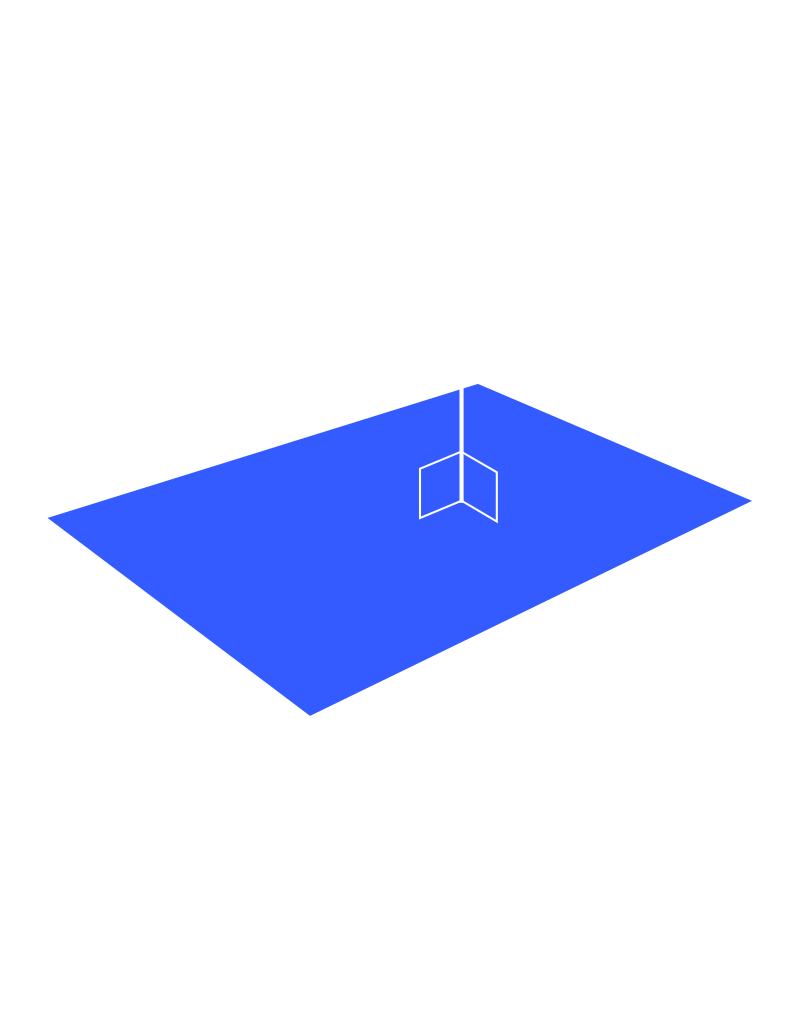
\includegraphics[scale=0.1]{./figures/Normal_vectors2.png}
\end{center}
\vfill
\begin{emptytitle}
    Given a point $P_0$ and a nonzero vector $\vec{n}$, there is
    a unique plane containing $P_0$ and orthogonal to $\vec{n}$.
\end{emptytitle}
}
%-------------- end slide -------------------------------%}}}
%-------------- start slide -------------------------------%{{{ 26
\begin{frame}[fragile]
\begin{emptytitle}
    Consider a plane containing a point $P_0$
    and orthogonal to vector
    $\vec{n}$, and let $P$ be an arbitrary point on this plane.
\end{emptytitle}
\pause
\vfill
\begin{emptytitle}
    Then \[ \vec{n}\dotprod\overrightarrow{P_0P} = 0,\]
\end{emptytitle}
\pause
\vfill
\begin{emptytitle}
    or, equivalently,
    \[ \vec{n}\dotprod (\overrightarrow{0P}-\overrightarrow{0P_0}) = 0,\]
    and is a \alert{vector equation} of the plane.
\end{emptytitle}
\end{frame}
%-------------- end slide -------------------------------%}}}
%-------------- start slide -------------------------------%{{{ 27
\frame{
\begin{emptytitle}
    \[
	\vec{n}\dotprod
    (\overrightarrow{0P}-\overrightarrow{0P_0}) = 0
    \quad\Longleftrightarrow\quad
	\vec{n}\dotprod \overrightarrow{0P}=
    \vec{n}\dotprod\overrightarrow{0P_0}
    \]
    \pause
    \vspace{-1em}
    \begin{center}
    by setting $P_0=P_0(x_0,y_0,z_0)$, $P=P(x,y,z)$, $\vec{n}=\left[\begin{array}{ccc} a & b & c \end{array}\right]^T$
    \end{center}
    \pause
    \[
    \Longleftrightarrow \quad
    \left[\begin{array}{c}
    a \\ b \\ c \end{array}\right]
    \dotprod
    \left[\begin{array}{c}
    x \\ y \\ z \end{array}\right]
    =
    \left[\begin{array}{c}
    a \\ b \\ c \end{array}\right]
    \dotprod
    \left[\begin{array}{c}
    x_0 \\ y_0 \\ z_0 \end{array}\right]
    \]
    \pause
    \[
    \Longleftrightarrow \quad
    ax+by+cz=ax_0+by_0+cz_0,\]
    \pause
    \vspace{-1em}
    \begin{center}
    setting $d=ax_0+by_0+cz_0$ --  a scalar
    \end{center}
    \pause
    \[
    \Longleftrightarrow \quad
    \boxed{ax+by+cz=d}\:,\mbox{ where }  a,b,c,d\in\RR.\]
    \pause
    \begin{center}
    This is the \alert{scalar equation} of the plane.
    \end{center}
  \end{emptytitle}
}
%-------------- end slide -------------------------------%}}}
%-------------- start slide -------------------------------%{{{ 28
\frame{
\begin{problem}
    Find an equation of the plane containing $P_0(1, -1, 0)$ and
    orthogonal to
    $\vec{n} =\left[\begin{array}{ccc}
    -3 & 5 & 2 \end{array}\right]^T$.
\end{problem}
\vfill
\pause
\begin{solution}
    A \alert{vector equation} of this plane is
    \[
	\left[\begin{array}{r}
	-3 \\ 5 \\ 2 \end{array}\right]
	\dotprod
	\left[\begin{array}{c}
	x-1 \\ y+1 \\ z \end{array}\right] = 0.\]
    \pause
    A \alert{scalar equation} of this plane is
    \[
    -3x+5y+2z=-3(1)+5(-1)+2(0) = -8,\]
    i.e., the plane has scalar equation
    \[ -3x + 5y +2z=-8.\]
\end{solution}
}
%-------------- end slide -------------------------------%}}}
%-------------- start slide -------------------------------%{{{ 29
\frame{
\begin{problem}
    Find the shortest distance from the point $P(2,3,0)$ to the plane
    with equation $5x+y+z=-1$, and find the point $Q$ on the plane
    that is closest to $P$.
\end{problem}
\vfill
\pause
\begin{solution}
    \begin{picture}(2,1.4)
	% \put(0.2,0.2){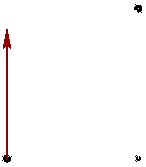
\includegraphics[scale=.7]{figures/vectors-18_copy.pdf}}
	\put(0.2,0.12){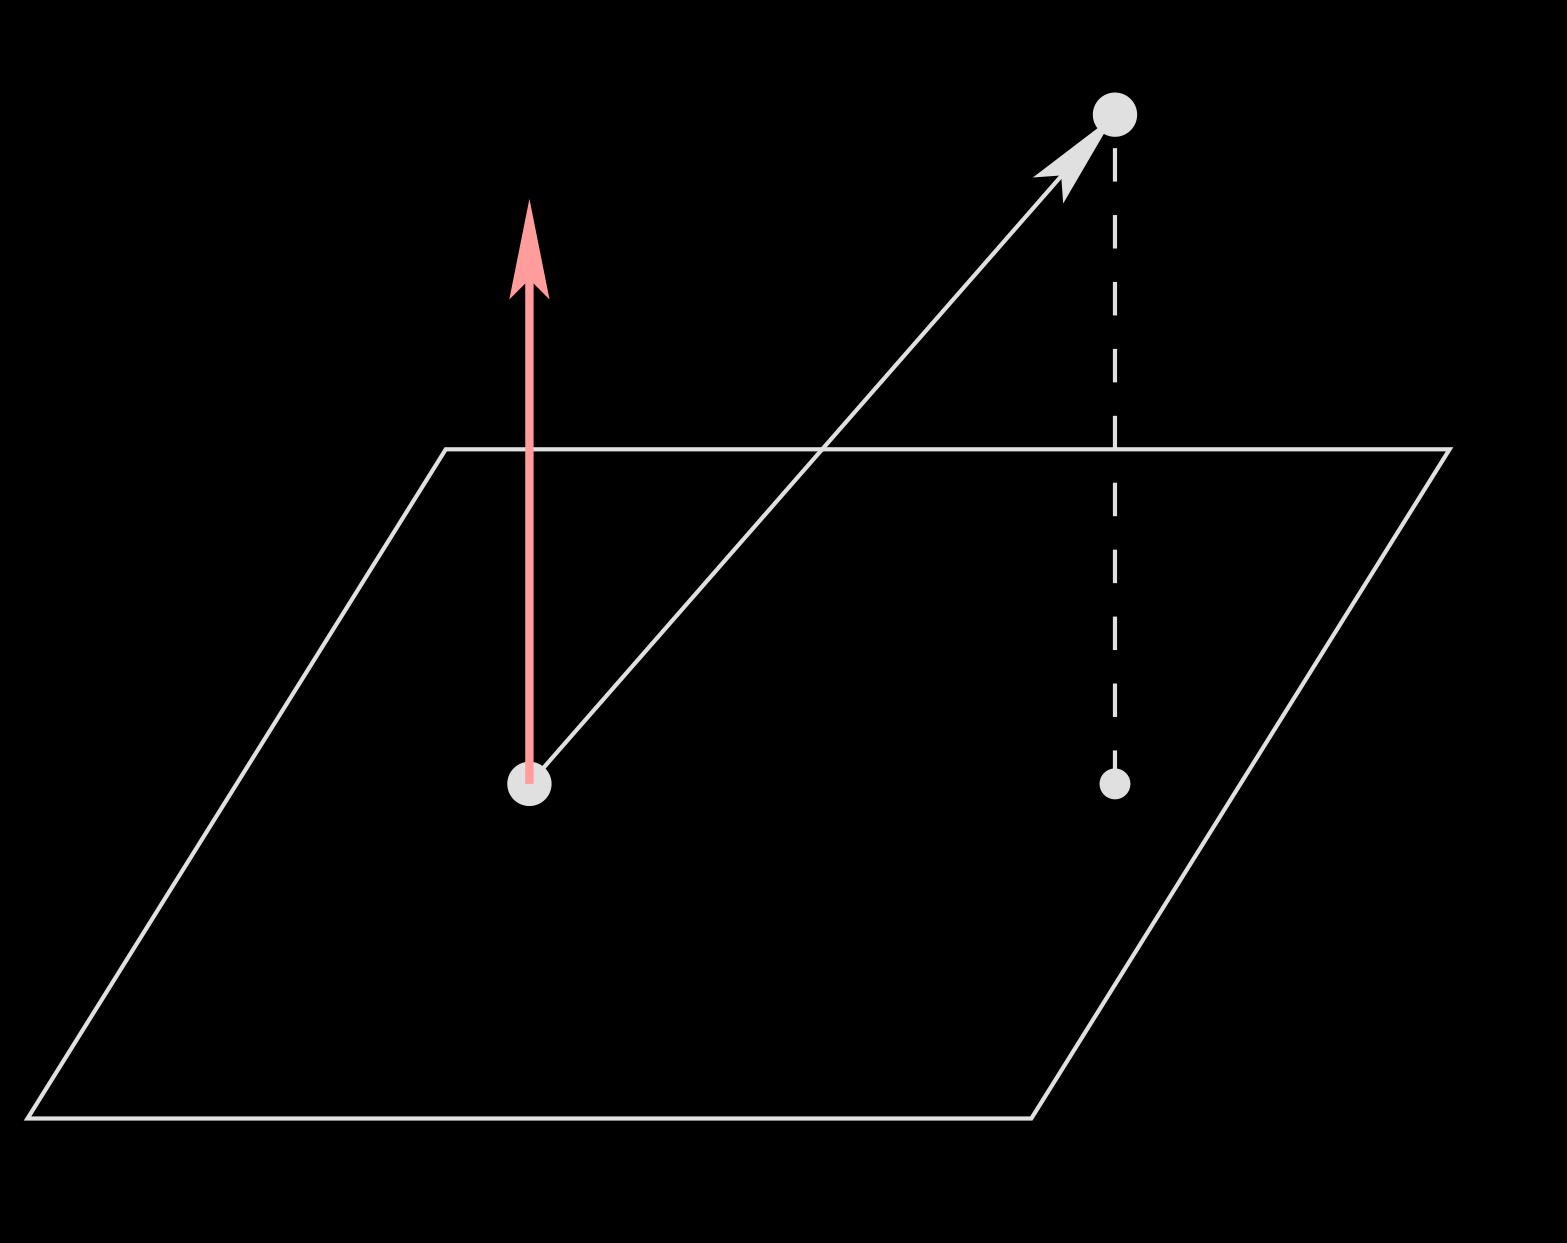
\includegraphics[scale=.065]{figures/vectors-18.png}}
	\put(0.6,0.4){\small $P_0$}
	\put(0.75,0.9){\small $\vec{n}$}
	\put(1.2,0.4){\small $Q$}
	\put(1.2,1.2){\small $P(2,3,0)$}
	\put(2.2,1.0){\small Pick an arbitrary point $P_0$ on the plane.}
	\put(2.2,0.7){\small Then
	$\overrightarrow{QP}=\proj_{\vec{n}}\overrightarrow{P_0P}$,}
	\put(2.3,0.5){$||\overrightarrow{QP}||$ is the shortest distance,}
	\put(2.3,0.3){and
	$\overrightarrow{0Q}=\overrightarrow{0P}-\overrightarrow{QP}$. }
    \end{picture}
    \pause

    $\vec{n}=\left[\begin{array}{ccc} 5 & 1 & 1 \end{array}\right]^T$.
    \pause
    Choose $P_0=P_0(0,0,-1)$.
    \bigskip
    \pause
    Then $$\overrightarrow{P_0P} = \left[\begin{array}{ccc} 2 & 3 & 1 \end{array}\right]^T$$
\end{solution}
}
%-------------- end slide -------------------------------%}}}
%-------------- start slide -------------------------------%{{{ 30
\frame{
\begin{solution}[continued]
\begin{picture}(2,1.3)
    \put(0.2,0.15){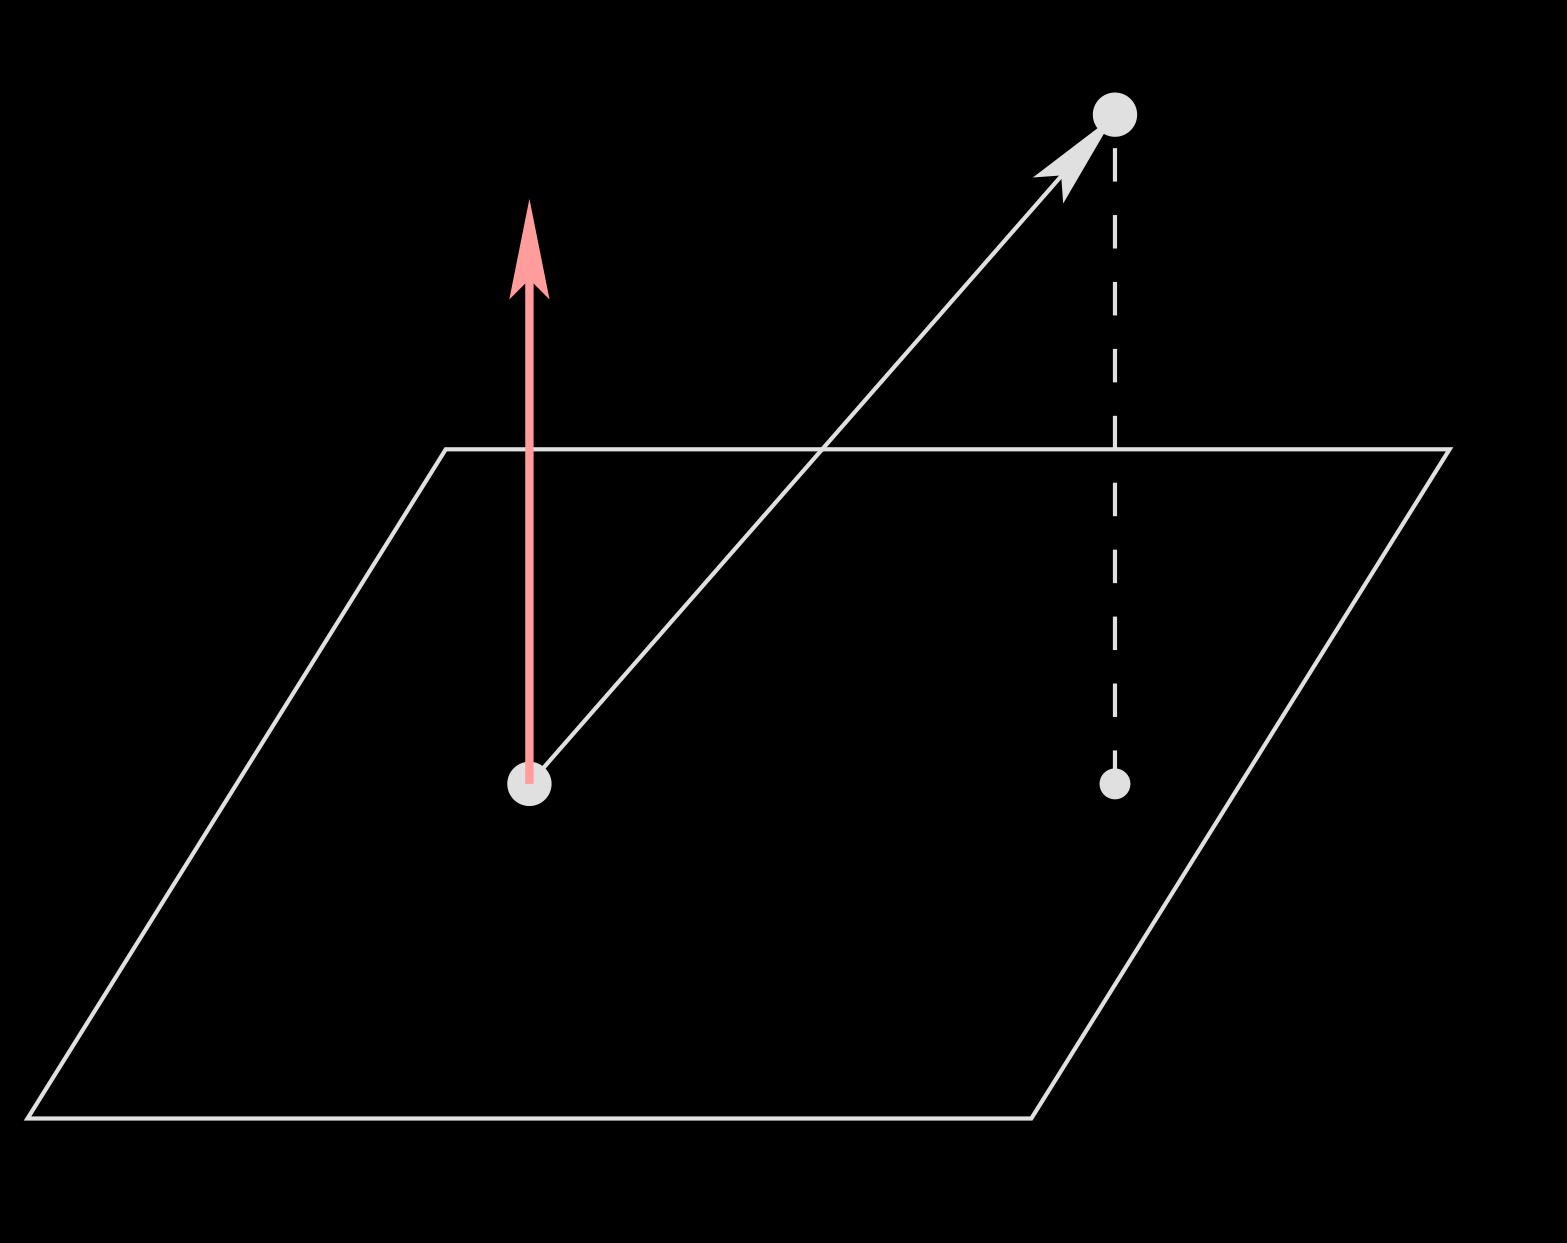
\includegraphics[scale=.065]{figures/vectors-18.png}}
    \put(0.6,0.4){\small $P_0$}
    \put(0.8,1.0){\small $\vec{n}$}
    \put(1.2,0.4){\small $Q$}
    \put(1.2,1.25){\small $P(2,3,0)$}
    \put(2.2,1.0){\small $\overrightarrow{P_0P}
	= \left[\begin{array}{ccc}
    2 & 3 & 1 \end{array}\right]^T$.}
    \put(2.2,0.7){\small $\vec{n}
	= \left[\begin{array}{ccc}
    5 & 1 & 1 \end{array}\right]^T$.}
\end{picture}
\vspace*{-.3in}
\uncover<2->{{\small
	\[ \overrightarrow{QP}=
	    \proj_{\vec{n}}\overrightarrow{P_0P}
	    =\frac{\overrightarrow{P_0P}\dotprod\vec{n}}{||\vec{n}||^2}
	    \vec{n}
	    =\frac{14}{27}
	    \left[\begin{array}{ccc}
	    5 & 1 & 1 \end{array}\right]^T.
\]}}
% \vspace*{-.2in}

\uncover<3->{{\small Since $||\overrightarrow{QP}||= \frac{14}{27}\sqrt{27}
	=\frac{14\sqrt{3}}{9}$, the shortest distance from $P$ to the plane
is $\frac{14\sqrt{3}}{9}$.}}
\bigskip

\uncover<4->{{\small
To find $Q$, we have
\begin{eqnarray*}
    \overrightarrow{0Q} = \overrightarrow{0P} - \overrightarrow{QP}
& = &
\left[\begin{array}{ccc}
2 & 3 & 0 \end{array}\right]^T -
\frac{14}{27}
\left[\begin{array}{ccc}
5 & 1 & 1 \end{array}\right]^T \\
& = & \frac{1}{27}
\left[\begin{array}{ccc}
-16 & 67 & -14 \end{array}\right]^T.
\end{eqnarray*}}
}

\uncover<5->{{\small
Therefore $Q=Q\left( -\frac{16}{27}, \frac{67}{27}, -\frac{14}{27}\right)$.}}
\end{solution}
}
%-------------- end slide -------------------------------%}}}
%-------------- start slide -------------------------------%{{{ 31
\begin{frame}[fragile]
   \begin{remark}
       Here is a general answer: the distance from $P\left(x_0,y_0,z_0\right)$ to the plane $ax+by+cz=d$ is
       \begin{align*}
	   \text{distance} = \frac{\left|ax_0+by_0+cz_0-d\right|}{\sqrt{a^2+b^2+c^2}}
       \end{align*}
   \end{remark}
\end{frame}
%-------------- end slide -------------------------------%}}}
\section[\textcolor{yellow}{}]{\textcolor{yellow}{Cross Product}}
%-------------- start slide -------------------------------%{{{ 32
\frame{
\frametitle{The Cross Product}
\pause
\begin{definition}
    Let $\vec{u}=\left[\begin{array}{ccc}
    x_1 & y_1 & z_1 \end{array}\right]^T$
    and
    $\vec{v}=\left[\begin{array}{ccc}
    x_2 & y_2 & z_2 \end{array}\right]^T$.
    Then
    \[
    \vec{u}\times\vec{v} =
    \left[\begin{array}{c}
	y_1z_2-z_1y_2 \\
	-(x_1z_2-z_1x_2) \\
	x_1y_2-y_1x_2
    \end{array}\right].\]
\end{definition}
\vfill\pause

\begin{center}
    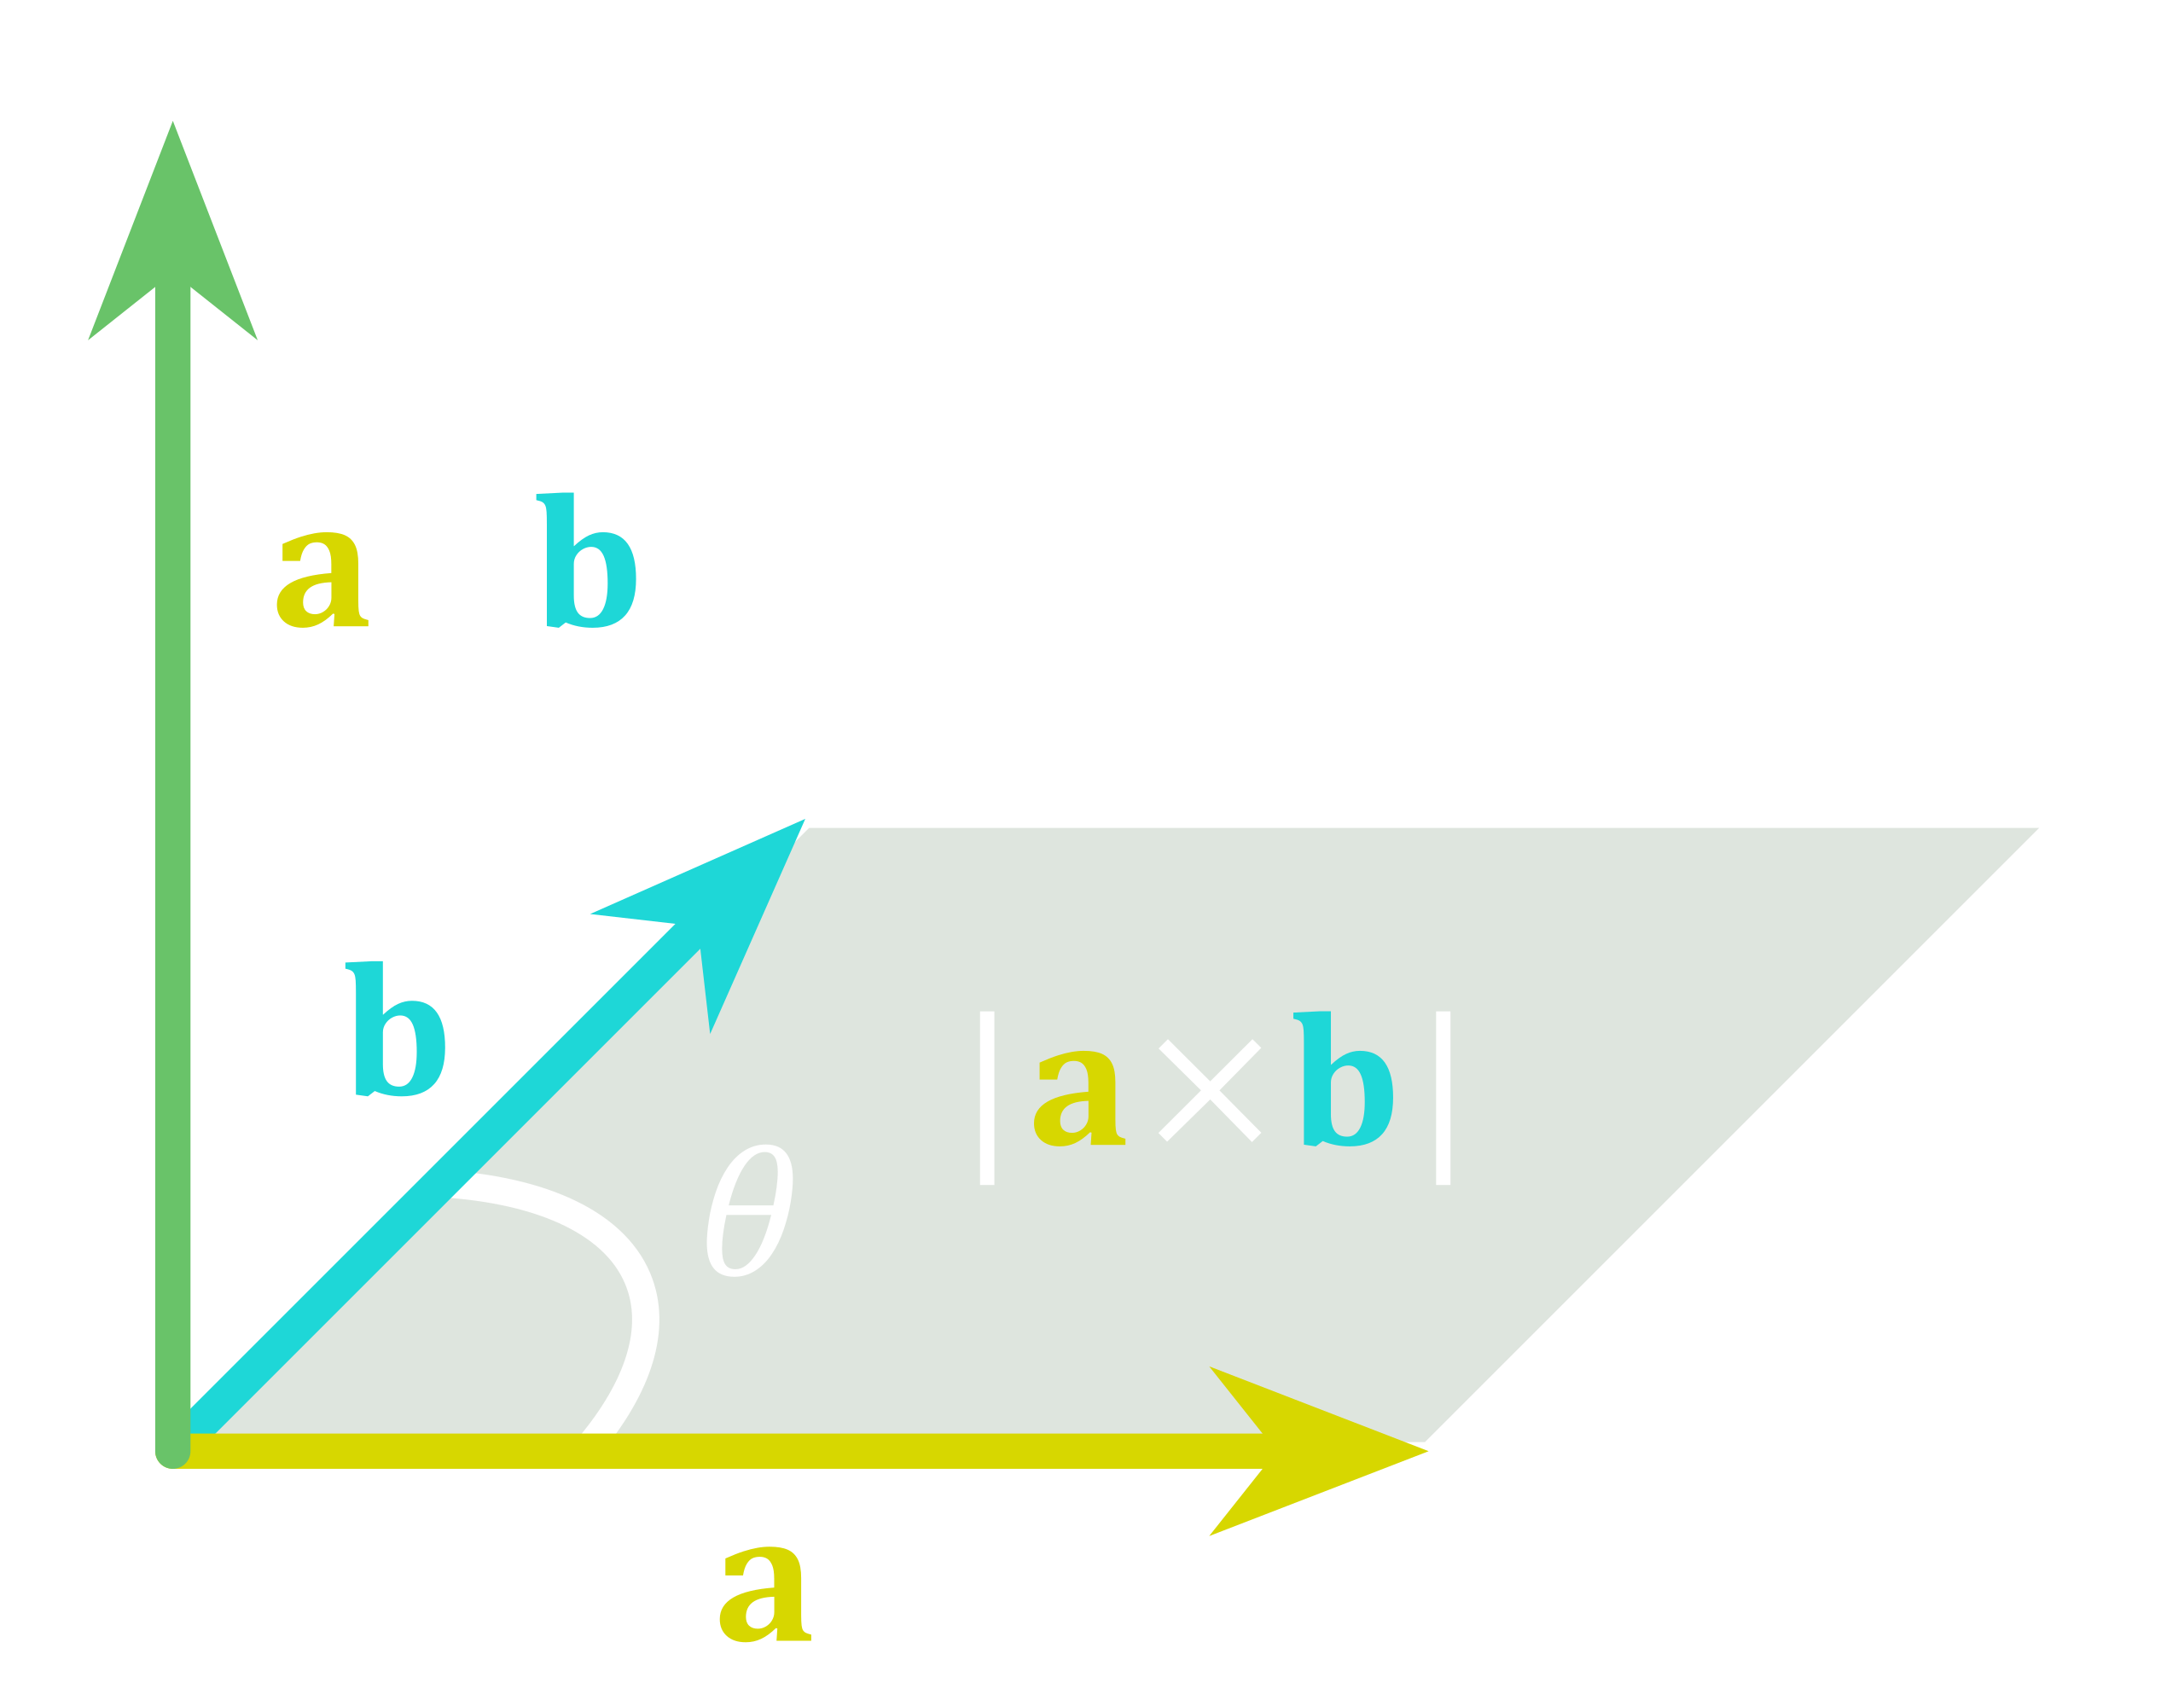
\includegraphics[scale=0.03]{./figures/Cross_product_parallelogram.png}
\end{center}

\begin{remark}
$\vec{u}\times\vec{v}$ is a vector:
\begin{itemize}
    \item Direction: orthogonal to both $\vec{u}$ and $\vec{v}$.
    \item Size: the area of the corresponding parallelogram.
\end{itemize}
\end{remark}

}
%-------------- end slide -------------------------------%}}}
%-------------- start slide -------------------------------%{{{ 33
\begin{frame}[fragile]
\begin{remark}
    \alert{A mnemonic device:}
    \[
    \vec{u}\times\vec{v} =
    \left|\begin{array}{ccc}
	\vec{i} & x_1 & x_2 \\
	\vec{j} & y_1 & y_2 \\
	\vec{k} & z_1 & z_2
    \end{array}\right|,
    \mbox{ where }
    \vec{i} =
    \left[\begin{array}{c}
    1 \\ 0 \\ 0 \end{array}\right],
    \vec{j} =
    \left[\begin{array}{c}
    0 \\ 1 \\ 0 \end{array}\right],
    \vec{k} =
    \left[\begin{array}{c}
    0 \\ 0 \\ 1 \end{array}\right].
    \]
    Or equivalently,
    \[
    \vec{u}\times\vec{v} =
    \left|\begin{array}{ccc}
	\vec{i} & \vec{j} & \vec{k} \\
	 x_1    & y_1     & z_1     \\
	 x_2    & y_2     & z_2
    \end{array}\right|
    \]
\end{remark}
\end{frame}
%-------------- end slide -------------------------------%}}}
%-------------- start slide -------------------------------%{{{ 34
\frame{
\begin{theorem}
    Let $\vec{v}, \vec{w}\in\RR^3$.
    \begin{enumerate}
    \item<2-> $\vec{v}\times\vec{w}$ is orthogonal to both $\vec{v}$ and $\vec{w}$.
    \item<3-> If $\vec{v}$ and $\vec{w}$ are both nonzero, then $\vec{u}\times\vec{w}=\vec{0}$ if and only if $\vec{v}$ and $\vec{w}$ are parallel.
    \end{enumerate}
\end{theorem}
}
%-------------- end slide -------------------------------%}}}
%-------------- start slide -------------------------------%{{{ 35
\frame{
\begin{problem}
    Find all vectors orthogonal to both
    $\vec{u}=\left[\begin{array}{ccc}
    -1 & -3 & 2 \end{array}\right]^T$
    and
    $\vec{v}=\left[\begin{array}{ccc}
    0 & 1 & 1 \end{array}\right]^T$.
    {\small (We previously solved this using the \alert{dot product}.)}
\end{problem}
\vfill
\pause
\begin{solution}
    \[
	\vec{u}\times\vec{v} =
	\left|\begin{array}{crr}
	    \vec{i} & -1 & 0 \\
	    \vec{j} & -3 & 1 \\
	    \vec{k} & 2  & 1
	\end{array}\right|
	= -5\vec{i} +\vec{j}-\vec{k}
	= \left[\begin{array}{r} -5 \\ 1 \\ -1 \end{array}\right].
    \]
    \vspace*{-.1in}

    Any scalar multiple of $\vec{u}\times\vec{v}$ is also
    orthogonal to both $\vec{u}$ and $\vec{v}$, so
    \[ t\left[\begin{array}{r} -5 \\ 1 \\ -1 \end{array}\right], \quad\forall t\in\RR, \]
    gives all vectors orthogonal to both $\vec{u}$ and $\vec{v}$.
    \\[1em]

    (Compare this with our earlier answer.)
\end{solution}
}
%-------------- end slide -------------------------------%}}}
%-------------- start slide -------------------------------%{{{ 36
\frame{
\begin{problem}
    Given two lines
    \[
	L_1:
	\left[\begin{array}{c}
	x \\ y \\ z \end{array}\right]
	=
	\left[\begin{array}{r}
	3 \\ 1 \\ -1 \end{array}\right]
	+
	s\left[\begin{array}{r}
	1 \\ 1 \\ -1 \end{array}\right]
	\quad\text{and}\quad
	L_2:
	\left[\begin{array}{c}
	x \\ y \\ z \end{array}\right]
	=
	\left[\begin{array}{r}
	1 \\ 2 \\ 0 \end{array}\right]
	+
	t\left[\begin{array}{r}
	1 \\ 0 \\ 2 \end{array}\right],
    \]
    \begin{itemize}
	\item[A.]
	    Find the shortest distance between $L_1$ and $L_2$.
	\item[B.]
	    Find the points $P$ on $L_1$ and $Q$ on $L_2$ that are closest together.
    \end{itemize}
\end{problem}
}
%-------------- end slide -------------------------------%}}}
%-------------- start slide -------------------------------%{{{ 37
\begin{frame}[fragile]
\begin{solution}
    \begin{picture}(2,1.3)
	\put(0.18,0.18){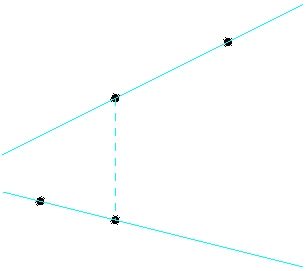
\includegraphics[scale=.6]{figures/vectors-19_copy.pdf}}
	\put(0.25,0.3){\scriptsize $P_2$}
	\put(0.6,0.25){\scriptsize $Q$}
	\put(0.6,0.95){\scriptsize $P$}
	\put(1.07,0.9){\scriptsize $P_1$}
	\put(1.4,1){Choose $P_1(3,1,-1)$ on $L_1$ and
	$P_2(1,2,0)$ on $L_2$.}
	\put(1.4,0.6){
	    Let $\vec{d}_1=
	    \left[\begin{array}{r}
	    1 \\ 1 \\ -1 \end{array}\right]$
	    and $\vec{d}_2=
	    \left[\begin{array}{r}
	1 \\ 0 \\ 2 \end{array}\right]$ denote direction }
	\put(1.4,0.2){vectors for $L_1$ and $L_2$, respectively.}
\end{picture}
\end{solution}

\end{frame}
%-------------- end slide -------------------------------%}}}
%-------------- start slide -------------------------------%{{{ 38
\frame{
\begin{picture}(2,1.3)
    \put(0.14,0.16){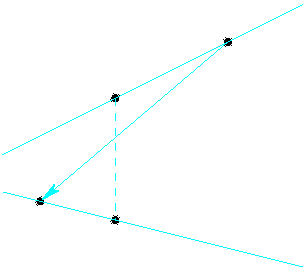
\includegraphics[scale=.65]{figures/vectors-20_copy.pdf}}
    \put(0.05,0.3){\scriptsize $P_2(1,2,0)$}
    \put(0.6,0.25){\scriptsize $Q$}
    \put(0.6,0.95){\scriptsize $P$}
    \put(1.07,0.95){\scriptsize $P_1(3,1,-1)$}
    \put(2.0,0.8){\scriptsize $\vec{d}_1=
	\left[\begin{array}{r}
	1 \\ 1 \\ -1 \end{array}\right]$,
	$\vec{d}_2=
	\left[\begin{array}{r}
    1 \\ 0 \\ 2 \end{array}\right]$}
    \put(2.0,0.4){\scriptsize The shortest distance between
    $L_1$ and $L_2$ is the length}
    \put(2.05,0.25){\scriptsize of the projection of
	$\overrightarrow{P_1P_2}$ onto
    $\vec{n}=\vec{d}_1\times\vec{d}_2$.}
\end{picture}

\uncover<2->{
    {\small
	\[
	    \overrightarrow{P_1P_2}=
	    \left[\begin{array}{r}
	    -2 \\ 1 \\ 1 \end{array}\right]
	    \quad\text{and}\quad
	    \vec{n}=
	    \left[\begin{array}{r}
	    1 \\ 1 \\ -1 \end{array}\right]
	    \times
	    \left[\begin{array}{r}
	    1 \\ 0 \\ 2 \end{array}\right]
	    =
	    \left[\begin{array}{r}
	    2 \\ -3 \\ -1 \end{array}\right]
\]}}

\uncover<3->{
    {\small
	\[ \proj_{\vec{n}}\overrightarrow{P_1P_2}
	    =
	    \frac{\overrightarrow{P_1P_2}\dotprod\vec{n}}{||\vec{n}||^2}\vec{n},
	    \quad\text{and}\quad
	    ||  \proj_{\vec{n}}\overrightarrow{P_1P_2}||
	    =
	    \frac{|\overrightarrow{P_1P_2}\dotprod\vec{n}|}{||\vec{n}||}.
\]}}

\uncover<4->{
    {\small
	Therefore, the shortest distance between $L_1$ and $L_2$ is
$\frac{|-8|}{\sqrt{14}}=\frac{4}{7}\sqrt{14}$.}}
}
%-------------- end slide -------------------------------%}}}
%-------------- start slide -------------------------------%{{{ 39
\frame{
    \small{
	% \begin{example}[continued]
	\textcolor{lgtblue}{Solution B.}

	\begin{picture}(2,1.3)
	    \put(0.2,0.2){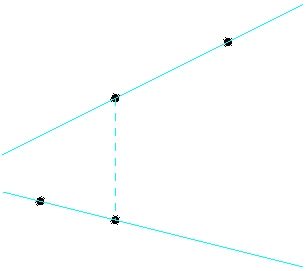
\includegraphics[scale=.6]{figures/vectors-19_copy.pdf}}
	    \put(0.05,0.3){\scriptsize $P_2(1,2,0)$}
	    \put(0.6,0.25){\scriptsize $Q$}
	    \put(0.6,0.95){\scriptsize $P$}
	    \put(1.07,0.95){\scriptsize $P_1(3,1,-1)$}
	    \put(2.0,1.2){\scriptsize
		$\vec{d}_1=
		\left[\begin{array}{r}
		1 \\ 1 \\ -1 \end{array}\right]$,
		$\vec{d}_2=
		\left[\begin{array}{c}
	    1 \\ 0 \\ 2 \end{array}\right]$;}
	    \put(2.0,0.7){\scriptsize
		$\overrightarrow{0P}=
		\left[\begin{array}{c}
		3+s \\ 1 + s \\ -1 -s \end{array}\right]$
	    for some $s\in\RR$;}
	    \put(2.0,0.2){\scriptsize
		$\overrightarrow{0Q}=
		\left[\begin{array}{c}
		1+t \\ 2  \\ 2t \end{array}\right]$
	    for some $t\in\RR$.}
	\end{picture}

	\uncover<2->{
	    Now $\overrightarrow{PQ}=\left[\begin{array}{ccc}
	    -2-s+t & 1-s & 1+s+2t \end{array}\right]^T$ is orthogonal
	    to both $L_1$ and $L_2$, so
	    \[ \overrightarrow{PQ}\dotprod\vec{d}_1 = 0
		\quad\text{and}\quad
	\overrightarrow{PQ}\dotprod\vec{d}_2 = 0,\]}
	\uncover<3->{i.e.,
	    \begin{eqnarray*}
		-2-3s-t &= & 0 \\
		s + 5t & = & 0.
	\end{eqnarray*}}

	\uncover<4->{This system has unique solution $s=-\frac{5}{7}$
	and $t=\frac{1}{7}$.}
	\uncover<5->{Therefore,
	    \[ P=P\left(\frac{16}{7}, \frac{2}{7}, -\frac{2}{7}\right)
		\quad\text{and}\quad
	    Q=Q\left(\frac{8}{7}, 2, \frac{2}{7}\right).\]
	    \vspace*{-.15in}
	}
	% \end{example}
}}
%-------------- end slide -------------------------------%}}}
%-------------- start slide -------------------------------%{{{ 40
\frame{

{\small
The shortest distance between $L_1$ and $L_2$ is
$||\overrightarrow{PQ}||$.
Since
\[ P=P\left(\frac{16}{7}, \frac{2}{7}, -\frac{2}{7}\right)
\quad\text{and}\quad
Q=Q\left(\frac{8}{7}, 2, \frac{2}{7}\right),\]

\uncover<2->{
\[ \overrightarrow{PQ}
=
\frac{1}{7}\left[\begin{array}{r}
8 \\ 14 \\ 2 \end{array}\right]
-
\frac{1}{7}\left[\begin{array}{r}
16 \\ 2 \\ -2 \end{array}\right]
=
\frac{1}{7}\left[\begin{array}{r}
-8 \\ 12 \\ 4 \end{array}\right],
\]}

\uncover<3->{
and
\[ ||\overrightarrow{PQ}|| =
\frac{1}{7}\sqrt{224}=\frac{4}{7}\sqrt{14}.\]
}

\uncover<4->{
Therefore the shortest distance between $L_1$ and $L_2$
is $\frac{4}{7}\sqrt{14}$.}
}}
%-------------- end slide -------------------------------%}}}
\section[\textcolor{yellow}{}]{\textcolor{yellow}{Shortest Distances}}
%-------------- start slide -------------------------------%{{{ 41
\frame{
\frametitle{Shortest Distances}
\pause

\begin{problem}[ Challenge Problem ]
    Write yourself a plan to find the shortest distance in $\R^3$ between either a point, line or plane, to either a point, line or plane.
\end{problem}
}
%-------------- end slide -------------------------------%}}}
%-------------- start slide -------------------------------%{{{ 42
\begin{frame}[fragile]
\frametitle{Point-point distance}
\pause
\begin{emptytitle}
    If $P$ and $Q$ are two points, then $d\left(P,Q\right) = |\overrightarrow{PQ}|$.
\end{emptytitle}
\vfill
\begin{center}
    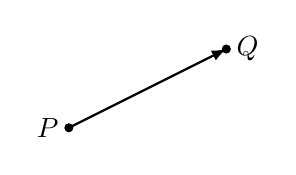
\begin{tikzpicture}[scale=1, transform shape]
        \tikzset{>=latex}
        \coordinate (Q) at (2,1);
        \coordinate (P) at (0,0);
        \draw[->,thick] (P) node [left] {$P$}-- (Q) node [right] {$Q$};
        \filldraw (P) circle (0.05);
        \filldraw (Q) circle (0.05);
    \end{tikzpicture}
\end{center}
\end{frame}
%-------------- end slide -------------------------------%}}}
%-------------- start slide -------------------------------%{{{ 43
\begin{frame}[fragile]
\frametitle{Point-plane distance}
\pause
\begin{emptytitle}
If $P$ is a point and $\Sigma: \vec{n}\cdot \vec{x}=d$ is a plane
containing a point $Q$, then
\begin{align*}
  d\left(P,\Sigma\right) = \frac{\left|\overrightarrow{PQ}\cdot \vec{n} \right|}{|\vec{n}|}
\end{align*}
\end{emptytitle}
\vfill
\begin{center}
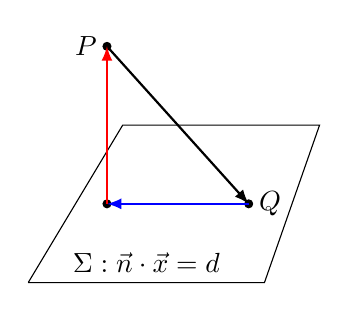
\begin{tikzpicture}[scale=1, transform shape]
    \tikzset{>=latex}
    \coordinate (P) at (1,3);
    \coordinate (Q) at (2.8,1);
    \coordinate (N) at (1,1);
    \draw (0,0) -- (1.2, 2) -- (3.7,2) -- (3,0) -- (0,0);
    \draw[->,thick] (P) node [left] {$P$} -- (Q) node [right] {$Q$};
    \filldraw (P) circle (0.05);
    \filldraw (Q) circle (0.05);
    \filldraw (N) circle (0.05);
    \draw [blue,->,thick] (Q) -- (N);
    \draw [red,->,thick] (N) -- (P);
    \node at (1.5,0.25) {$\Sigma: \vec{n}\cdot \vec{x}=d$};
\end{tikzpicture}
\end{center}
\end{frame}
%-------------- end slide -------------------------------%}}}
%-------------- start slide -------------------------------%{{{ 44
\begin{frame}[fragile]
\frametitle{Point-line distance}
\pause
\begin{emptytitle}
    If $P$ is a point and $L$ is a line $\vec{r}(t)=Q + t \vec{u}$, then
    \begin{align*}
        d\left(P,L\right) = \frac{\left|\overrightarrow{PQ}\times \vec{u} \right|}{|\vec{u}|}
    \end{align*}
\end{emptytitle}
\vfill
\begin{center}
\begin{tikzpicture}[scale=1, transform shape]
    \tikzset{>=latex}
    \coordinate (P) at (1,3);
    \coordinate (Q) at (3.2,1);
    \coordinate (N) at (1,1);
    % \draw (0,0) -- (1.2, 2) -- (3.7,2) -- (3,0) -- (0,0);
    \draw (-0.5,1) -- (4,1) node [right] {$L$};
    \draw[->] (P) node [above] {$P$} -- (Q) node [below] {$Q$};
    \filldraw (P) circle (0.05);
    \filldraw (Q) circle (0.05);
    \filldraw (N) circle (0.05);
    \draw [blue,->,thick] (Q) -- (N);
    \draw [red,->,thick] (N) -- (P);
    % \node at (1.5,0.25) {$\Sigma: \vec{n}\cdot \vec{x}=0$};
\end{tikzpicture}
\end{center}
\end{frame}
%-------------- end slide -------------------------------%}}}
%-------------- start slide -------------------------------%{{{ 45
\begin{frame}[fragile]
\frametitle{Line-line distance}
\pause
\begin{emptytitle}
    If $L$ is a line $\vec{r}(t)=Q + t \vec{u}$ and $M$ is another line
    $\vec{s}=P+t \vec{v}$, then
    \begin{align*}
      d\left(L,M\right) = \frac{\left|\overrightarrow{PQ}\cdot \left(\vec{u} \times \vec{v}\right) \right|}{|\vec{u} \times \vec{v}|}
    \end{align*}
\end{emptytitle}
\vfill
\begin{center}
\begin{tikzpicture}[scale=1, transform shape]
    \tikzset{>=latex}
    \coordinate (P2) at (1.5,3.6);
    \coordinate (P) at (1,3);
    \coordinate (Q) at (3.2,1);
    \coordinate (N) at (1,1);
    % \draw (0,0) -- (1.2, 2) -- (3.7,2) -- (3,0) -- (0,0);
    \draw (-0.5,1) -- (4,1) node [right] {$L$};
    \draw (-0,1.8) -- (2,4.2) node [right] {$M$};
    \draw[->] (P2) node [above] {$P$} -- (Q) node [below] {$Q$};
    \filldraw (P) circle (0.05);
    \filldraw (P2) circle (0.05);
    \filldraw (Q) circle (0.05);
    \filldraw (N) circle (0.05);
    \draw [blue,->,thick] (Q) -- (N);
    \draw [red,->,thick] (N) -- (P);
    % \node at (1.5,0.25) {$\Sigma: \vec{n}\cdot \vec{x}=0$};
\end{tikzpicture}
\end{center}
\end{frame}
%-------------- end slide -------------------------------%}}}
%-------------- start slide -------------------------------%{{{ 46
\begin{frame}[fragile]
\frametitle{Plane-plane distance}
\pause
\begin{emptytitle}
    If $\Sigma: \vec{n}\cdot \vec{x}=d$ and $\Theta: \vec{n} \cdot \vec{x} =e$ are two parallel planes, then
    \begin{align*}
        d\left(\Sigma,\Theta\right) =\frac{|e-d|}{|\vec{n}|}
    \end{align*}
\end{emptytitle}
\vfill
\begin{center}
    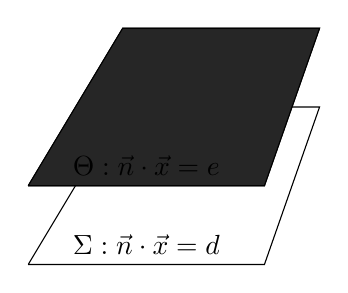
\begin{tikzpicture}[scale=1, transform shape]
    \tikzset{>=latex}
    \coordinate (P2) at (1.5,3.6);
    \coordinate (P) at (1,3);
    \coordinate (Q) at (3.2,1);
    \coordinate (N) at (1,1);
    \draw (0,0) -- (1.2, 2) -- (3.7,2) -- (3,0) -- (0,0);
    \node at (1.5,0.25) {$\Sigma: \vec{n}\cdot \vec{x}=d$};
    \filldraw [gray!30!black] (0,1) -- (1.2, 3) -- (3.7,3) -- (3,1) -- (0,1);
    \draw (0,1) -- (1.2, 3) -- (3.7,3) -- (3,1) -- (0,1);
    \node at (1.5,1.25) {$\Theta:\vec{n}\cdot \vec{x}=e$};
    \end{tikzpicture}
\end{center}
\end{frame}
%-------------- end slide -------------------------------%}}}
\end{document}
